\section{Visualizing High-dimensional Data}

When we measure a system with more than two parameters, the result becomes
high-dimensional data that cannot be easily mapped to a 2D figure. One
can select a subset of results to present but then we are going back
to the question of which settings we should choose. Therefore, in
this work, we set our goal to be presenting all data.

\begin{figure}[t]
    \centering
    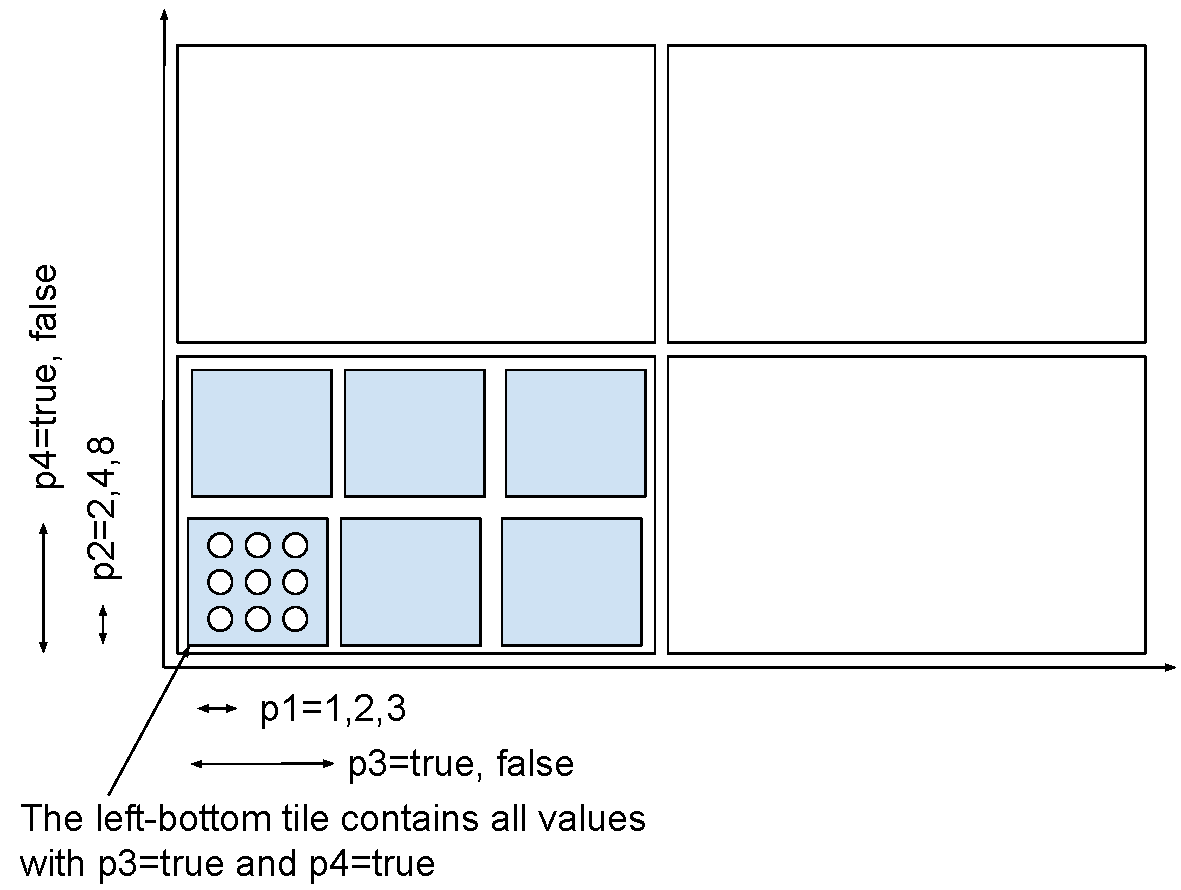
\includegraphics[width=0.45\textwidth]{tiledgraph}
    \caption{Tiled Heat Map.}
    \vspace{-.1in}
    \label{fig:tiledgraph}
\end{figure}

To achieve this goal, we design and develop a tool to visualize high-dimensional
data on a figure called Tiled Heat Map (Figure~\ref{fig:tiledgraph}):
assuming the system has $n$ parameters from $p_1$
to $p_n$, in the first iteration, our tool picks two parameters (e.g., $p_1$ and $p_2$) and groups all
data with the same $p_3$ to $p_n$; then it is able to draw each group
on a 2D figure called a ``tile'' since each group only contains two parameters $p_1$ and $p_2$.
In the second iteration, our tool picks two additional parameters (e.g., $p_3$ and $p_4$)
and groups tiles with the same $p_5$ to $p_n$ into a super-tile. It repeats
this procedure until it covers all parameters (the last iteration may just pick one parameter). 
Our tool uses Matplotlib~\cite{matplotlib} as its plotting interface. 
Section~\ref{sec:cases} shows some real
Tiled Heat Maps we build.

\vspace{-.1in}
\paragraph{Order of parameters.}
Our tool needs to choose parameters in each iteration.
Among all the possible choices, we try to choose the one that causes
the final figure to be ``smooth'' for easy reading (i.e., large values are close
to each other and small values are close to each other). Formally, we define the following metric
to measure how ``smooth'' a figure is, assuming there are $n$ points in the figure,
and each point has a coordinate $(x_i, y_i)$ and a value $v_i$.

\begin{definition}

    $smoothness = |SpearmanCorrelation(D, V)|$
    
, in which

$D=\{\forall (i,j), d_{ij} = |x_i-x_j|+|y_i-y_j| \}$

$V=\{\forall (i,j), v_{ij} = |v_i-v_j|\}$


\end{definition}

% \todo{Miao, add a short description about Pearson Correlation}
% Pearson's correlation coefficient~\cite{pearsonCorr} is used to measure the linear correlation between two sets of data.
We use Spearman's correlation coefficient~\cite{spearmanCorr}, which is the Pearson's correlation~\cite{pearsonCorr} between two rank variables, to measure how well the relationship between $D$ and $V$ can be described using a monotonic function. We choose Spearman's correlation over Pearson's because the latter measures linearity, while we only care about monotonicity here.

Intuitively, a high smoothness value means the value difference between two points
is highly correlated with the distance between them. In other words,
points with very different values
are far away from each other and points with close values are close to each other,
which is exactly what we want.

Our tool tries all the possible orders of parameters to compute the smoothness of each order
and chooses the one with the highest smoothness. If the figure contains many points,
our tool samples a subset of them to compute the smoothness value. Assuming the target system has $p$ parameters, there
is a total of $p!$ choices: with a small $p$, iterating all choices is feasible: with a 
bigger $p$, we probably need to go for heuristic solutions. In our experiments, we
find iterating all is feasible.

\vspace{-.1in}
\paragraph{Choosing the value and color of each point.} 
The Tiled Heat Map can be used to present different types of values, such as the
raw throughput, the improvement of one system over another, etc.

In the Tiled Heat Map, we use a color
to represent the value of each point. 
By default, our tool first finds the minimal and maximal values, and
then evenly distributes all values among gray color \#CECECE to \#0A0A0A (we observe
colors very close to full black or white are hard to distinguish, so we try to avoid them).
However, just like most graph plotting tools, our tool allows
the user to specify a color for a value range manually.
In this paper, we use gray colors to meet
the requirement of the conference, and using more colors can often create
a more readable version.

\vspace{-.1in}
\paragraph{Limitations.}
As shown in the next section, we find the Tiled Heat Map is good at presenting the overall
trend about how parameter values (or a combination of parameter values) can affect
system performance. However, it is not very good at presenting the absolute value of
each data point or comparing values with a small difference (e.g., 10\%). Therefore,
we propose the Tiled Heat Map as a complement to traditional line or bar graphs.
Furthermore, although the Tiled Heat Map can typically show more information on
the same area, its capability is still limited by the number of pixels we can have:
when viewing it on a computer, this problem can be addressed by zooming in/out, which we find helpful, but
when printing it on paper, there is eventually going to be a limit.
Finally, we have tried the Tiled Heat Map on data with at most five dimensions
and it is likely that more dimensions will make the figure harder to read.

%\vspace{-.1in}
%\paragraph{Suggestions.}
%While our community has always required figures in a publication to be readable
%when printed on a black-white printer and without a magnifier, which is
%very understandable, we argue it is eventually limiting the capability
%of presenting the results from extensive evaluation. We suggest our community
%to consider the possibility of allowing large colored figures, maybe as
%supplemental materials, for readers who are interested.


